% \clearpage

\section{Results}

\subsection{Covariance Matrix and Predictors Relationship}
The degree of the linear relationship between two variables may be measured using the covariance coefficients $(p)$. It ranges from -1 to +1, where large positive and negative values indicates positively and negatively correlated data,respectively. Its absolute magnitude measures the degree of redundancy. If the covariance is close to zero, the data is uncorrelated~\cite{Kuhn2013}.

\begin{table}[htbp]
  \caption{Covariance threshold analysis.}
  \begin{center}
  \begin{tabular}{|c|c|}
          \hline 
          $|p| \geq$ & Related Pairs\\
          \hline
          $0.75$ & 25\\
          \hline
          $0.90$ & 14 \\
          \hline
  \end{tabular}
\label{tab:Covariance}
\end{center}
\end{table}

From the obtained covariance matrix, we observe that 14 predictors pairs present strong correlation, greater than 0.9. It indicates that we can reduce the data dimensionality, since these pairs carry redundancy.

\begin{figure}[htbp!]
  \centerline{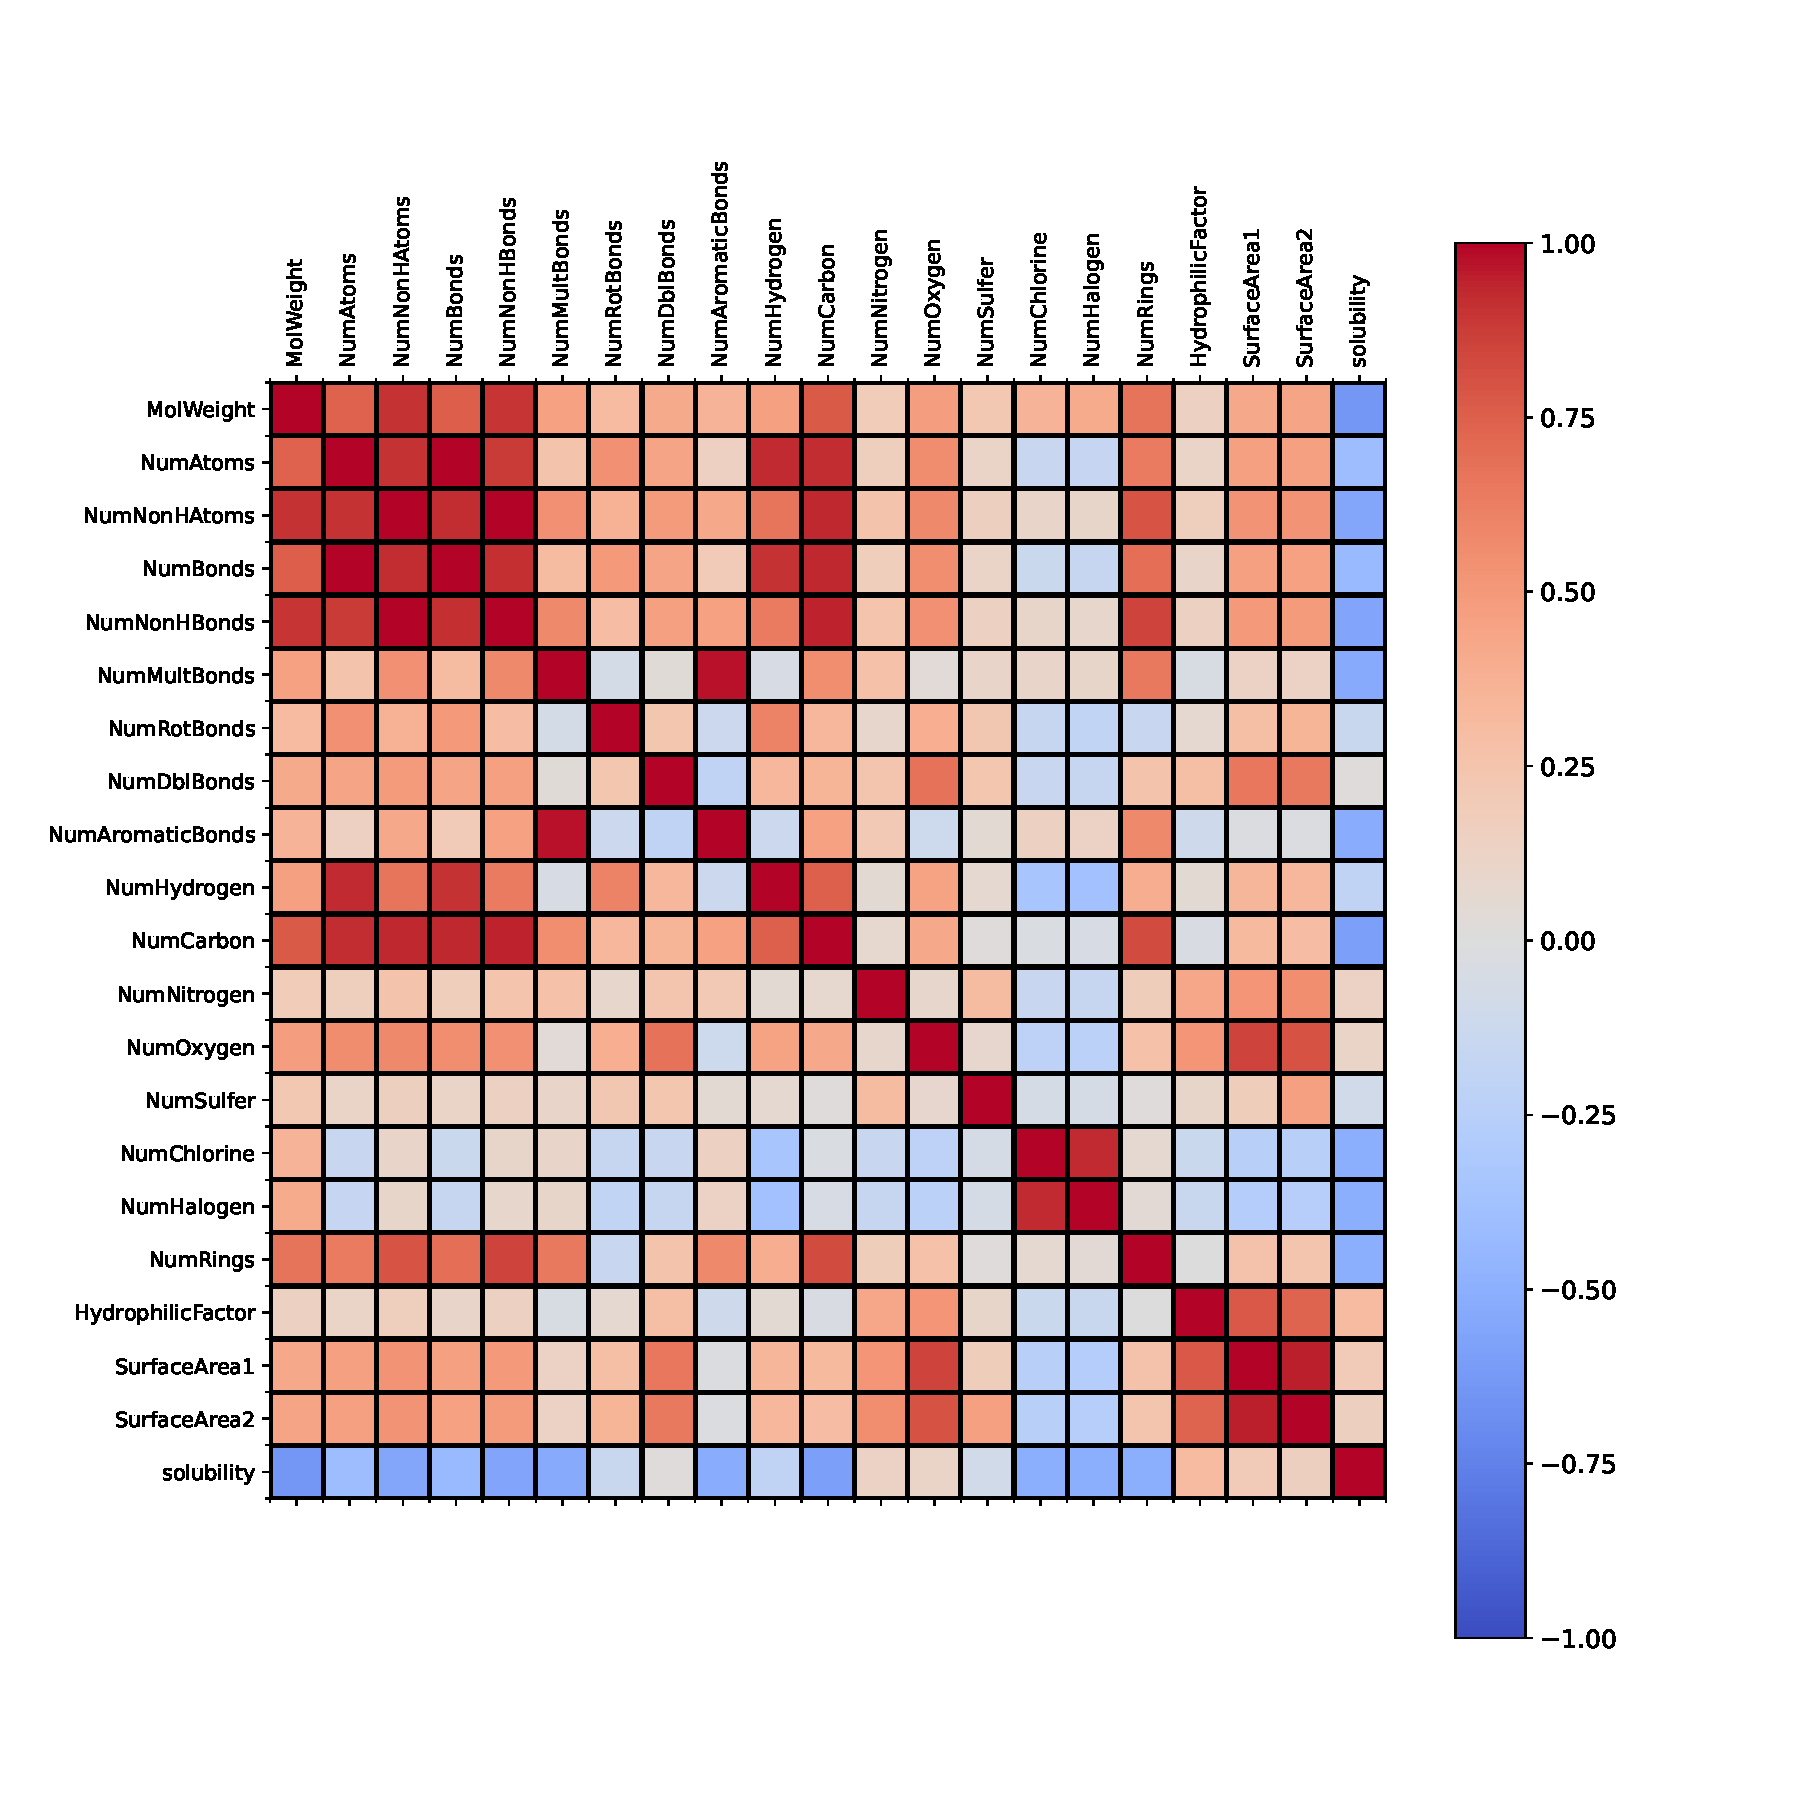
\includegraphics[width=0.55\textwidth]{../../code/hw2/figures/1-correlation_matrix.pdf}}
  \caption{Correlation Matrix presented as a Heatmap.}
  \label{fig:1-correlation_matrix}
\end{figure}

In order to provide data covariance in a understandable approach, we compute the covariance matrix and present it is a heatmap for visualization simplicity. Fig.~\ref{fig:1-correlation_matrix} shows that various predictors are strongly correlated, mainly positive.

\begin{figure}[htbp!]
  \centerline{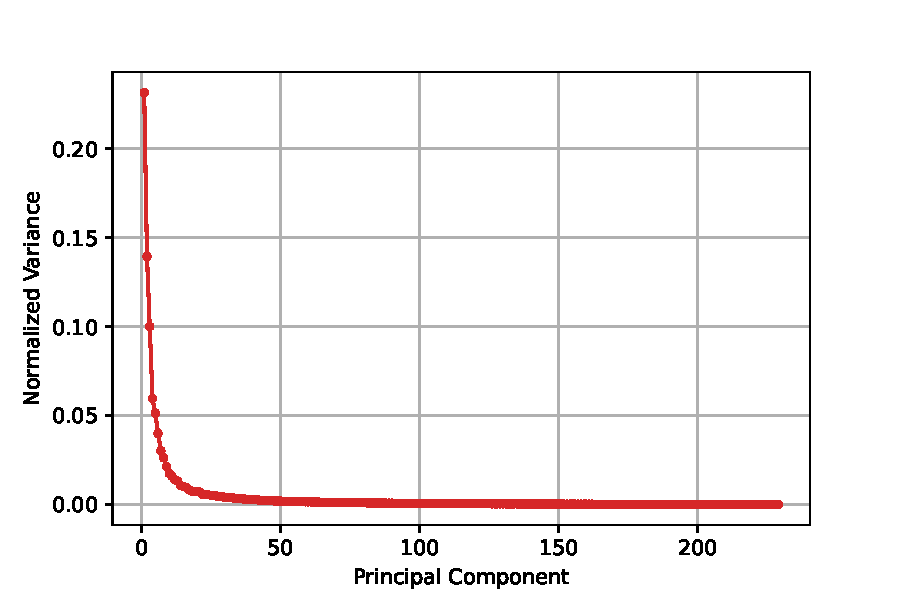
\includegraphics[width=0.52\textwidth]{../../code/hw2/figures/0-PCA-screeplot.pdf}}
  \caption{Screeplot showing the normalized variance, i.e, relevance, of each Principal Component.}
  \label{fig:0-PCA-screeplot}
\end{figure}

We can see in Fig.~\ref{fig:0-PCA-screeplot}, the normalized variance, i.e, relevance on our context vs. the principal components (PC). We also present a cumulative curve, which shows that the first 6 PC carries more than 60\% of the variance, leading to 95\% with 60 PC, what we can interprete as only 60 columns, i.e, 26\% of this dataset preserve 95\% from the original information. It means dividing the complexity by 3 and improving the storage and processing cost.

\reviewUrgent{Linear Regression Model}

\begin{figure}[htbp!]
  \centerline{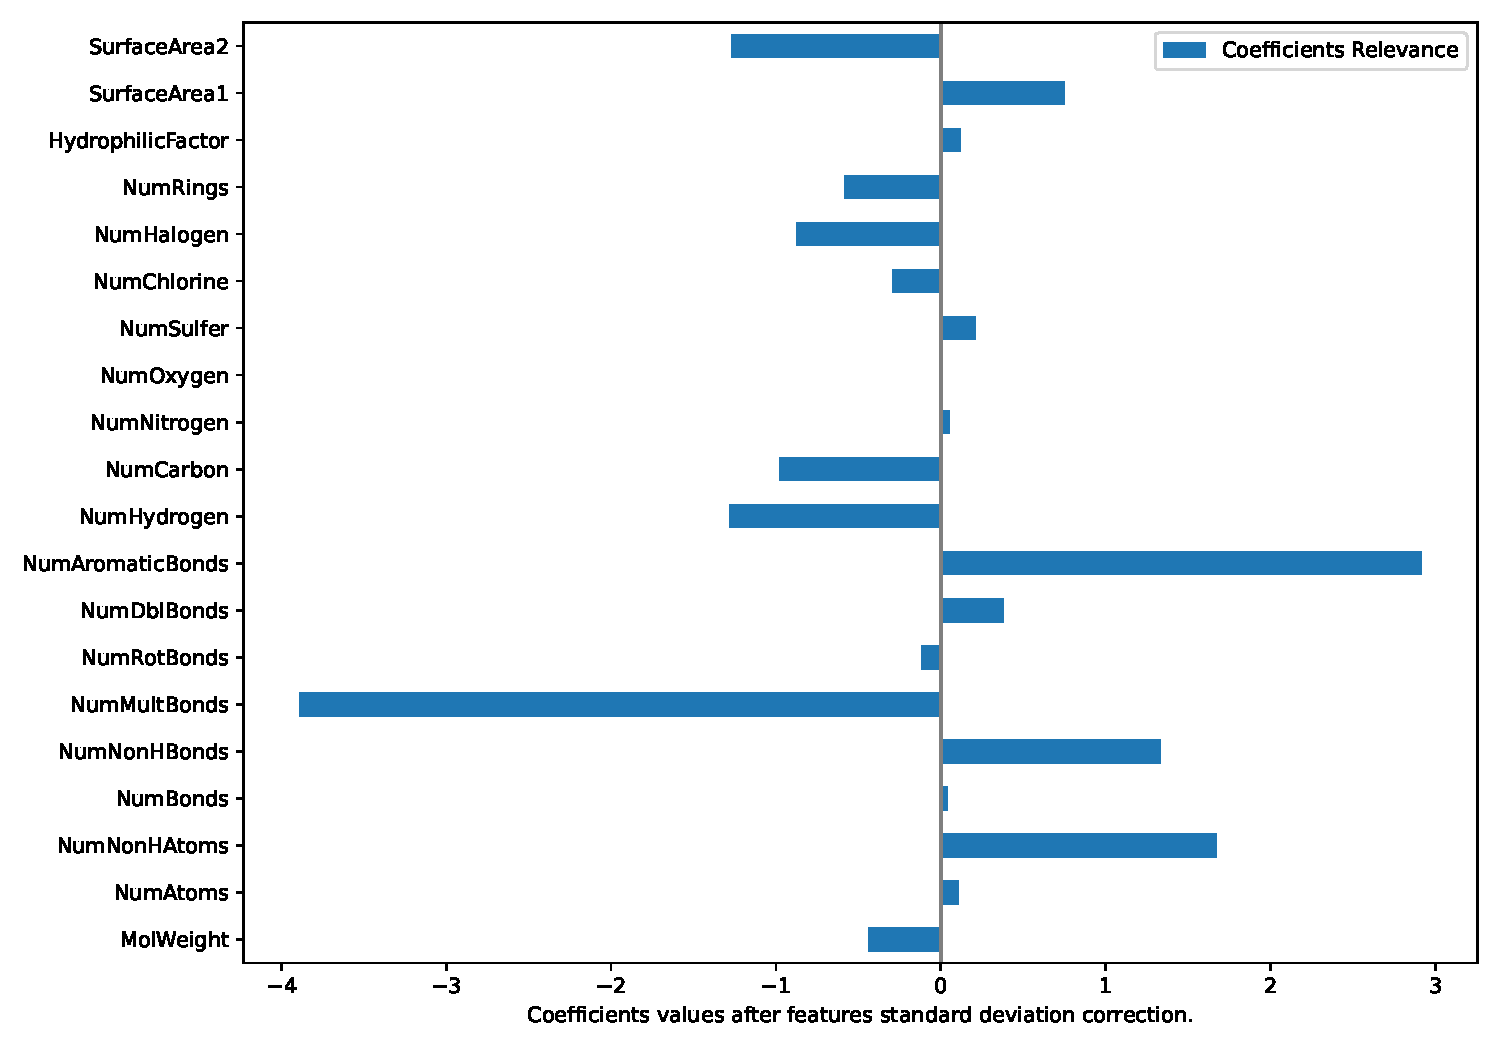
\includegraphics[width=0.5\textwidth]{../../code/hw2/figures/2-linear-regression-coefficients.pdf}}
  \caption{Linear regression coefficients.}
  \label{fig:2-linear-regression-coefficients}
\end{figure}


\reviewUrgent{Penalized Ridge Model}

\begin{figure}[htbp!]
  \centerline{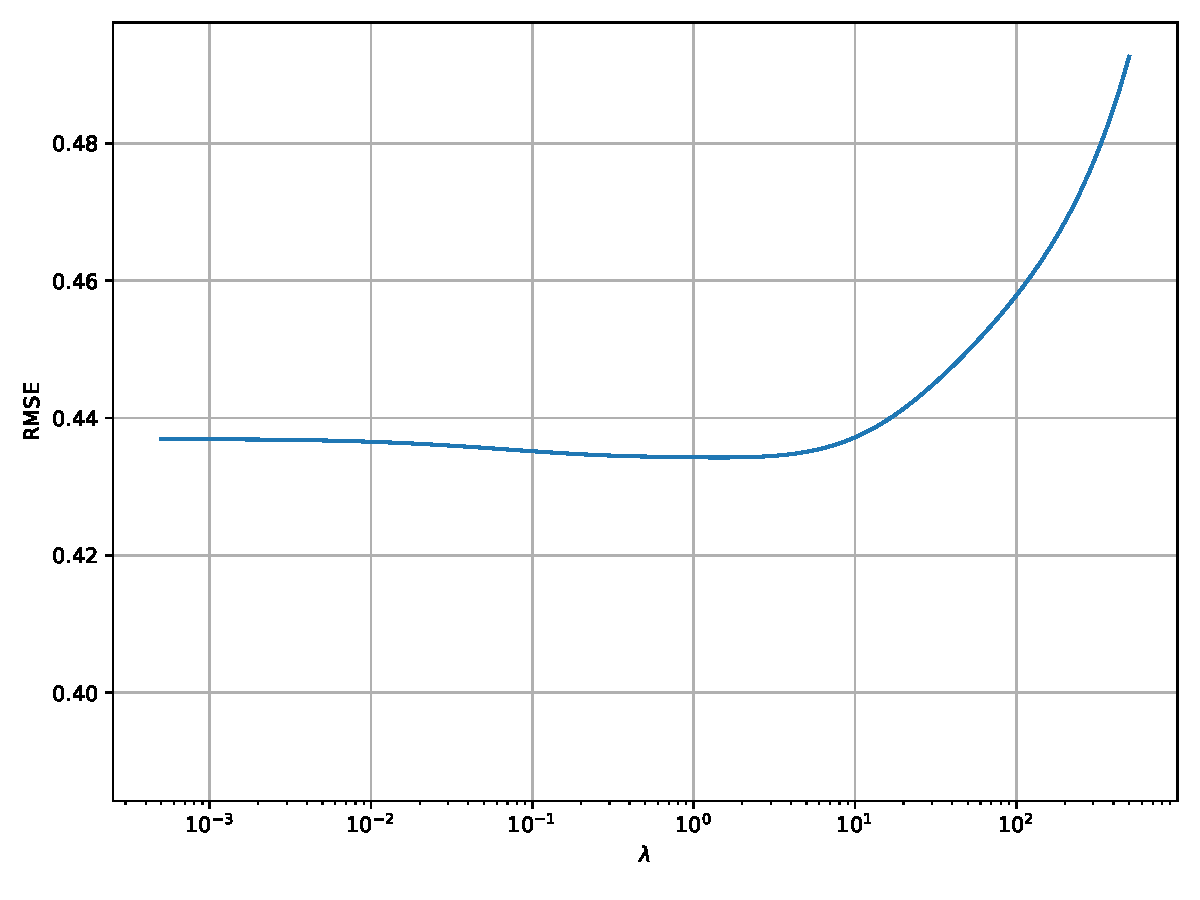
\includegraphics[width=0.5\textwidth]{../../code/hw2/figures/3-lambda-ridge.pdf}}
  \caption{$\lambda$ Parameter vs. RMSE for a Ridge Model.}
  \label{fig:3-lambda-ridge}
\end{figure}


\reviewUrgent{Principal Component Regression}

\begin{figure}[htbp!]
  \centerline{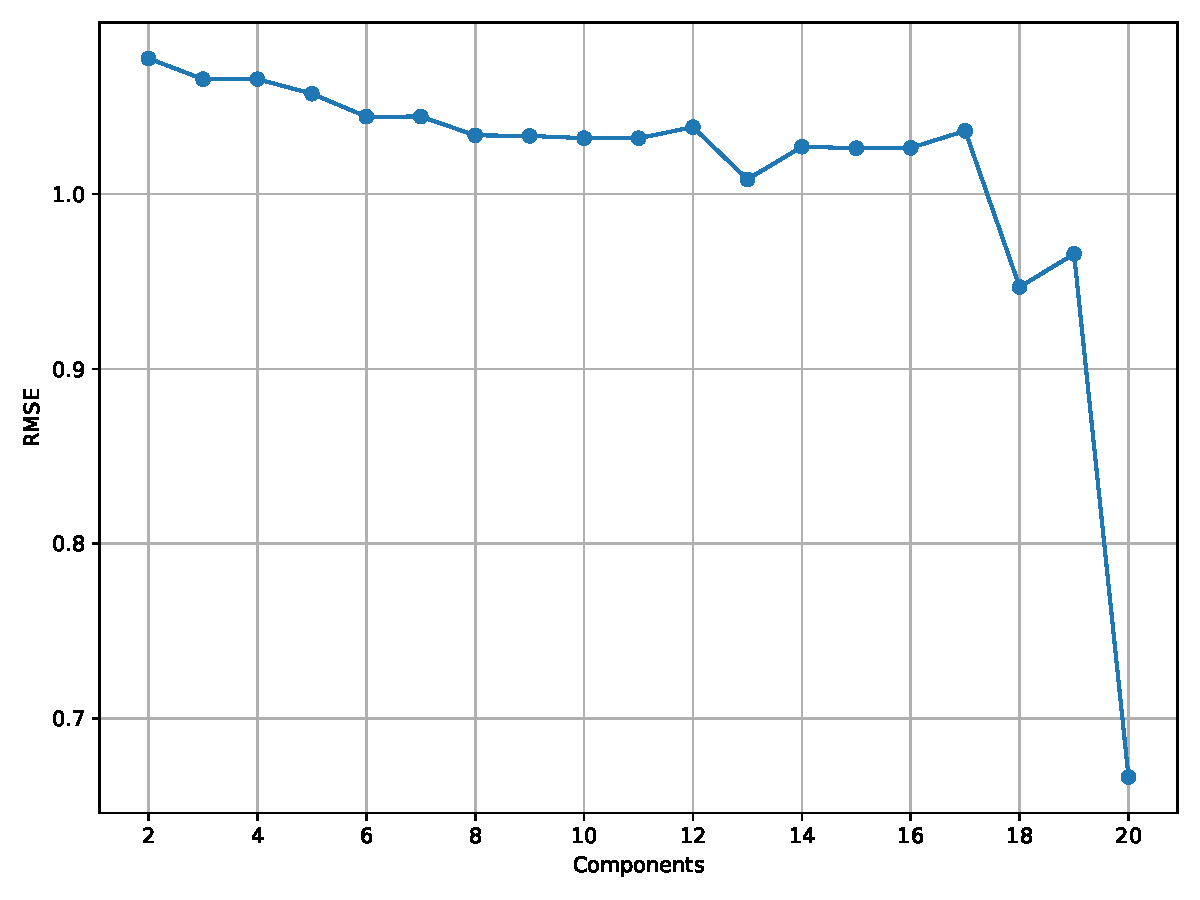
\includegraphics[width=0.5\textwidth]{../../code/hw2/figures/5-PCR-RMSE.pdf}}
  \caption{Components in the Model vs. RMSE for a PCR Model.}
  \label{fig:5-PCR-RMSE}
\end{figure}

\reviewUrgent{Partial Least Squares}

\begin{figure}[htbp!]
  \centerline{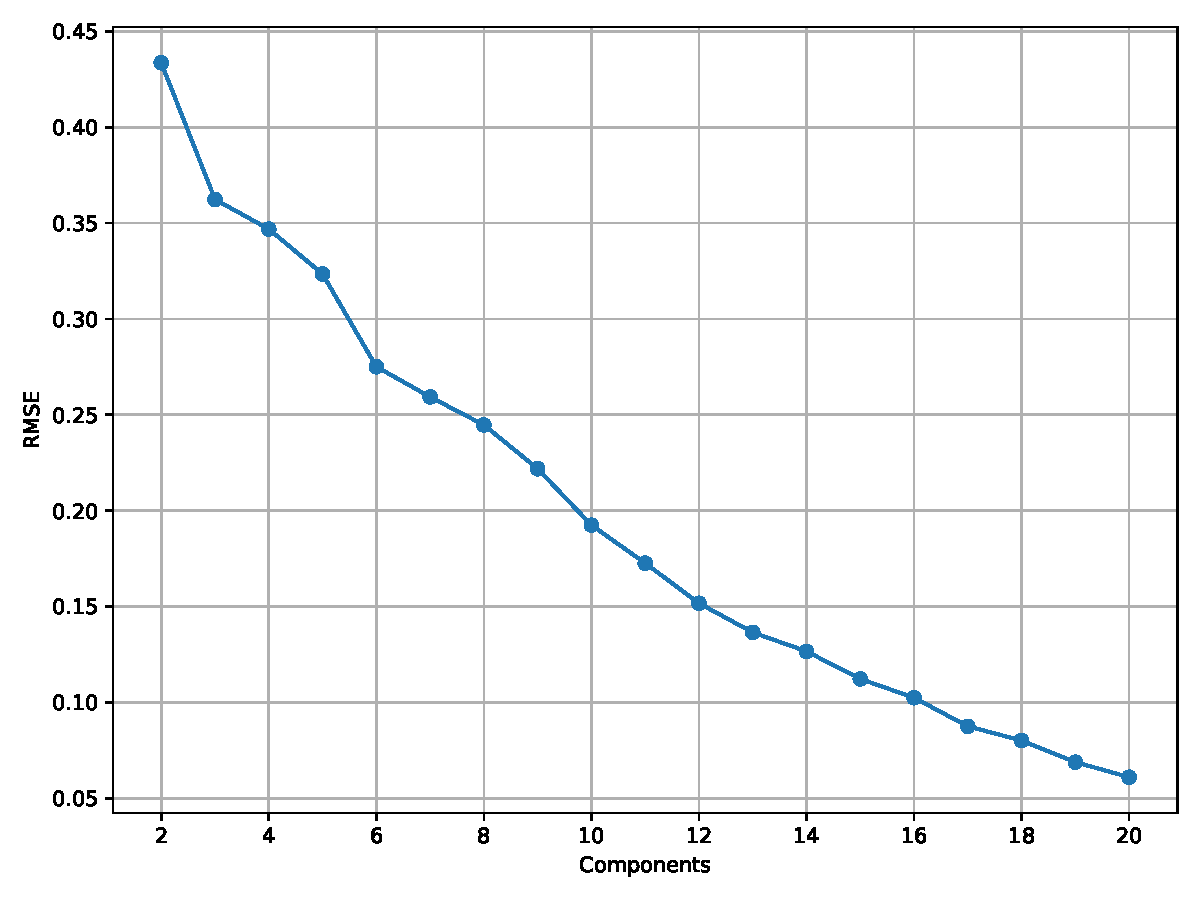
\includegraphics[width=0.5\textwidth]{../../code/hw2/figures/5-PLS-RMSE.pdf}}
  \caption{Components in the Model vs. RMSE for a PLS Model.}
  \label{fig:5-PLS-RMSE}
\end{figure}

% Inicialmente, é importante iniciar a análise do conjunto de dados verificando se existe a presença de algum nível de assimetria nas distribuições dos preditores. Caso existe assimetria no conjunto de dados é importante realizar uma transformação Box-Cox, aproximando o máximo possível a distribuição do conjunto de dados de uma distribuição normal.

% Após essas ações, foi necessário utilizar as ferramentas de centralização de média e normalização de variância para compensar a variedade nas unidades de medida associadas ao conjunto de preditores. Em seguida, é necessário analisar a linearidade dos preditores com as saídas por meio do ``scatter plot'' na figura (\ref{im:scatter}).

% % \begin{figure}[h]
% %     \centering
% %     \captionsetup{justification = centering,margin=1cm}
% %     \caption{ScatterPlot de um preditor linear e de um preditor não-linear, respectivamente.}
% %     \label{im:scatter}
% %     \includegraphics[width=0.4\textwidth, trim={0cm 14cm 13cm 1cm},clip]{images/ScatterPlot1.pdf}
% % \end{figure}

% Por meio da análise do ``scatter plot'' de todos os preditores é possível verificar que existe uma forte tendência a linearidade no conjunto de dados a ser modelado, embora exista alguns preditores que possuem uma tendência não linear ou uma tendência linear descontinuada em múltiplos intervalos. Sendo assim, é possível utilizar métodos de regressão linear a esse conjunto de dados e esperar uma precisão aceitável na predição.

% Finalmente, utiliza-se a  análise da componente principal(PCA) para reduzir a redundância possivelmente presente na matriz de dados. Logo a seguir é apresentada a matriz de correlação dos preditores:

% % \begin{figure}[h]
% %     \centering
% %     \captionsetup{justification = centering,margin=1cm}
% %     \caption{Matriz de Correlação dos Preditores}
% %     \label{fig:my_label}
% %     \includegraphics[width=0.5\textwidth, trim={4cm 4cm 0cm 7cm},clip]{images/MatrizCorrelacao.pdf}
% % \end{figure}

% %Parte 1

% \subsection{Regressão simples}

% Para a primeira abordagem foi implementado um modelo de regressão simples, utilizando a equação (\ref{eq:betas}). Os resultados foram razoavelmente satisfatórios, apresentando uma raiz de erro médio quadrático (RMSE) de 0,746, e a estatística $\text{R}^2$ em 0,872. O gráfico comparando os valores obtidos no modelo com os preditos está na figura (\ref{im:rsimples}).

% % \begin{figure}[h]
% %     \centering
% %     \captionsetup{justification = centering,margin=1cm}
% %     \caption{Regressão linear simples, aplicação direta}
% %     \includegraphics[width=0.3\textwidth]{images/LRTestScatterPlot.pdf}
% %     \label{im:rsimples}
% % \end{figure}

% É perceptível que uma boa aglomeração ao redor da linha central (que indica o valor previsto igual ao obtido), porém alguns pontos estão relativamente afastados, e esses acontecem com relativa frequência. Portanto seria interessante averiguar se com o mesmo tipo de modelo não se poderia reduzir esse erro, demonstrado que esses desvios não são apenas gerados pelo erro irredutível.

% Para tal, removeu-se os preditores altamente correlacionados e usou-se a validação cruzada, dividindo o conjunto de treino em 10 subgrupos. Aplicando o modelo aos grupos restantes no treino e validando-o no subgrupo removido. Ao final desse processo, foi selecionado o modelo com o melhor desempenho no conjunto de validação. Assim obtivemos o resultado da figura (\ref{im:rsimplescv}).

% % \begin{figure}[h]
% %     \centering
% %     \captionsetup{justification = centering,margin=1cm}
% %     \caption{Regressão linear simples, validação cruzada em 10 subgrupos}
% %     \includegraphics[width=0.3\textwidth]{images/TestLR10cv-9corr.pdf}
% %     \label{im:rsimplescv}
% % \end{figure}

% Durante a validação cruzada os melhores resultados foram RMSE = 0.698 e $\text{R}^2$ = 0,886, entretanto ao aplicar o modelo ao conjunto de teste obtivemos RMSE = 0,760 e $\text{R}^2$ = 0,867. Esse resultado nos permite suspeitar que provavelmente o processo de validação tenha enviesado demasiadamente o modelo, não permitindo um melhor desempenho no conjunto de teste. 
 
% %Parte 2
% \subsection{Modelo penalizado ``ridge''}

% O modelo penalizado utilizado em nossos experimentos foi o ``ridge regression'', que utiliza pesos quadráticos para compensar a varianças dos dados, e enviesando levemente os dados. Através de validação cruzada o valor ótimo do fator $\lambda$ foi determinado em 0,0286 (figura (\ref{im:lambda}) ), tendo dentro do conjunto de validação em RMSE = 0.676 e $\text{R}^2$ = 0.894. Esses resultados podem ser considerados mais interessantes que os valores obtidos na regressão simples, porém ao aplicar o modelo ao grupo de teste, a generalização do modelo não obteve resultados tão superiores a regressão simples, com RMSE = 0.720 e $\text{R}^2$ = 0.881. Apesar de que o desempenho no conjunto de teste não tenha sido tão superior, o resultado obtido no conjunto de validação indica que é provável haver uma melhor capacidade de generalização, tornando o modelo atrativo. 

% % \begin{figure}[h]
% %     \centering
% %     \captionsetup{justification = centering,margin=1cm}
% %     \caption{Determinação parâmetro $\lambda$}
% %     \includegraphics[width=0.3\textwidth]{images/lambda.pdf}
% %     \label{im:lambda}
% % \end{figure}

% %paRTE 3
% \subsection{PCR e PLS}

% Como ultima abordagem para o desenvolvimento do modelo preditivo, foram desenvolvidos dois modelos que utilizam a redução de dimensão, o PCR e o PLS. Foram aplicados os algorítimos para a aplicação dos modelos, então comparados as precisões a medida que o número de dimensões dos modelos aumentavam.

% % \begin{figure}[h]
% %     \centering
% %     \captionsetup{justification = centering,margin=1cm}
% %     \caption{RMSE em PCR}
% %     \includegraphics[width=0.3\textwidth]{images/ComponentsxRMSE_PCR.pdf}
% %     \label{im:pcr}
% % \end{figure}

% Interessante observar que na figura (\ref{im:pcr}) nem sempre que há um aumento de dimensões há uma diminuição considerável do RMSE, nos permitindo inferir que algumas dessas dimensões não apresentam correlação com saída como descrito anteriormente. Vale ressaltar que o valor inicial também é relativamente elevado, e mesmo com 40 dimensões, a precisão atingida durante a validação cruzada foi de RMSE = 0.872 e $\text{R}^2$ = 0.821, valores inferiores ao resultados a aplicação no conjunto de teste com regressão simples. O maior agravante foi que a aplicação no conjunto de teste teve um resultado pior, com RMSE = 0.898 e $\text{R}^2$ = 0.813. Esses resultados nos levaram a concluir que a regressão em componentes independentes não é adequada para o problema proposto visto que soluções mais simples fornecem resultados melhores.

% % \begin{figure}[h]
% %     \centering
% %     \captionsetup{justification = centering,margin=1cm}
% %     \caption{RMSE em PLS}
% %     \includegraphics[width=0.3\textwidth]{images/ComponentsxRMSE_PLS.pdf}
% %     \label{im:pls}
% % \end{figure}

% Em seguida aplicamos a regressão em PLS, e obtivemos resultados mais otimistas. Ao realizar a validação cruzada, ilustrado na figura (\ref{im:pls}), obtivemos uma curva mais optimizada e com um número muito menor de dimensões que a PCR. Vale ressaltar que principalmente ao se adicionar as primeiras dimensões, temos reduções expressivas no RMSE, que tende a se estabilizar a medida que se ultrapassa 17 dimensões. Durante a a validação o melhor resultado (dentre as 20 dimensões) se deu com 19 dimensões, com RMSE = 0.695 e $\text{R}^2$ = 0.887. Esses número são claramente mais desejáveis que os obtidos via PCR, quanto aos obtidos no grupo de teste foram, RMSE = 0.732 e $\text{R}^2$ = 0.877, esses são suavemente superiores aos obtidos via regressão simples, o quais dependendo do banco de dados final ou da precisão necessária, provavelmente não compensarão o esforço computacional extra.